\section{Numerical Tests}
\label{SEC_SCARC_Tests}
During the previous sections different Poisson solvers were presented, namely the structured FFT and different variants for structured \scarc{} as well as the unstructured \uglmat{} and \uscarc{}. To describe their algorithmic functionality, the pipe-shaped demonstration case {\ct poisson2d} from Figure \ref{FIG_basic_pipe_geometry} was used throughout the entire paper. 

Subsequently, this case will also be used as verification case to check how well the individual solvers can deal with internal obstructions and multi-mesh decompositions, and how quickly they can transmit global information.
To this end, air is blown into the domain whereby the inflow velocity is continuously varied within a range of 0 to 2 $m/s$ such that the flow pattern in the entire domain frequently changes. 
As will be seen below this special setting causes a very characteristic stair-like course of the pressure trace which is recorded in the middle pressure device up to a final simulation time of 0.5~s. 
%
The necessity to continuously adapt to varying global situations poses a particular challenge to the pressure solver and is intentionally used to analyze the related scalability of the different variants with respect to an increasing number of meshes.

\subsection{2D Poisson test case based on a subdivision into 4 meshes}
First, the {\ct poisson2d} geometry is subdivided into 4 meshes with a side length of 40~cm each. The single meshes are refined into $16^2$ cells corresponding to a grid resolution of 2.5~cm. The side length of the internal obstruction amounts to 10~cm. The resulting flow field at time $t=0.31$~s is illustrated in Figure \ref{FIG_scarc_poisson_four_flowfield}.


\begin{figure}[ht]
\begin{center}
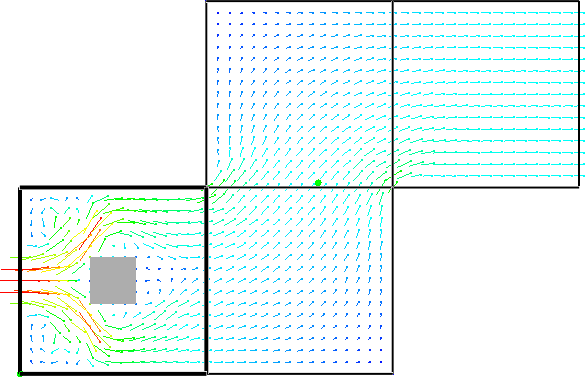
\includegraphics[width=0.55\textwidth]{\figPath/poisson2d_4mesh/poisson2d_4mesh_flowfield}
\end{center}
\caption[Flow field for a 4-mesh subdivision of the {\ct poisson2d} test case]{Flow field for a 4-mesh subdivision of the {\ct poisson2d} test case at $t=0.31$~s.}
\label{FIG_scarc_poisson_four_flowfield}
\end{figure}


Both structured solvers, FFT and \scarc{} were applied in two different versions, namely with the respective default velocity 0.0125 $m/s$ abbreviated as \fftdefault{} and \scarcdefault{}, and with a tight velocity tolerance of 0.00001 $m/s$ abbreviated as \ffttight{} and \scarctight{}.
No velocity tolerance had to be specified for the unstructured variants \uglmat{} and \uscarc{}. 
The measured pressure traces for these six different solvers are illustrated in Figure \ref{FIG_SCARC_poisson_four_trace}.

\begin{figure}[h]
\begin{center}
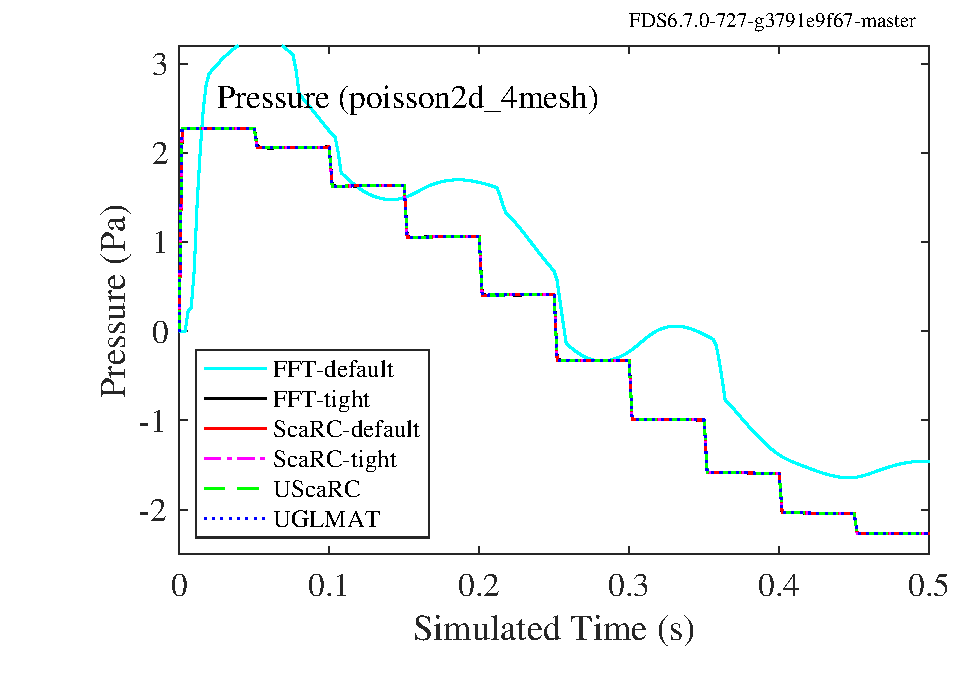
\includegraphics[width=3in]{\figPath/poisson2d_4mesh/poisson2d_4mesh_pres}
\end{center}
\caption[Pressure traces of the different pressure solvers for {\ct poisson2d} with 4 meshes]{Pressure traces of the different pressure solvers for a 4-mesh subdivision of the {\ct poisson2d} test case. }
\label{FIG_SCARC_poisson_four_trace}
\end{figure}

\newpage
As a globally operating direct method, \uglmat{} provides an exact solution to the global Poisson problem in each time step. Thus, its pressure trace is regarded as a reference solution for all other solvers.
%
Obviously \fftdefault{} (cyan) has troubles to map the pressure trace correctly while \scarcdefault{} (red) 
already seems to match exactly. Both are structured solvers which are not able to set the correct boundary values along the inner obstruction by design. However, this basically doesn't seem to carry much weight here, as can be seen for \scarcdefault{} for which the obstruction is the only possible error influence in this test case.

With a view to the constantly changing global velocity field, the multi-mesh decomposition seems to cause much more troubles 
which is reflected in the serpentine line of \fftdefault{}. The steady changes of the inflow conditions can only be spread across the entire domain by successive mesh-by-mesh communications. Thus, the new inflow information reaches the pressure device in the third mesh only with delay. Evidently, this cannot be sufficiently remedied by the default pressure iteration.

However, as observed for \ffttight{} (black), the tighter pressure iteration works great and is able to completely resolve these troubles leading to a correct pressure trace if only a higher number of pressure iterations is performed.
In contrast to this, there seems to be no reason at all to apply \scarctight{} (magenta dashed dotted) in this case. Since all \scarc{} variants provide correct transitions at mesh interfaces by design, the overall error influences are significantly less pronounced here.
Finally, \uscarc{} (green dashed) operates independently of all these effects and produces the same correct pressure trace as \uglmat{} (blue dotted).

So far, Figure (\ref{FIG_SCARC_poisson_four_trace}) reflects the accuracy which is achieved by the different solvers in the approximation of the pressure trace, but it does not say anything about the numerical effort required for this.
While for both unstructured solvers \uglmat{} and \uscarc{} only one pressure iteration is needed by construction, the structured variants require the execution of different numbers of pressure iterations until the respective velocity tolerance is met. 

To analyze this situation in more detail,  the achieved accuracies for the velocity errors, as displayed in Figure \ref{FIG_SCARC_poisson_four_velerror}, are set in relation to the number of pressure iterations required to reach them, as displayed in Figure \ref{FIG_SCARC_poisson_four_presite}.
Note, that Figure \ref{FIG_SCARC_poisson_four_velerror} only illustrates the velocity tolerances for the structured solvers because \uglmat{} and \uscarc{} achieve machine precision in the range of $10^{-16}$ by design which is omitted here to allow a more diversified view of the remaining solvers. Similarly, while the left plot in Figure \ref{FIG_SCARC_poisson_four_presite} compares the pressure iterations for all six solvers, the right plot omits \ffttight{} in order to give a more detailed overview of the others.

\begin{figure}[h]
\begin{center}
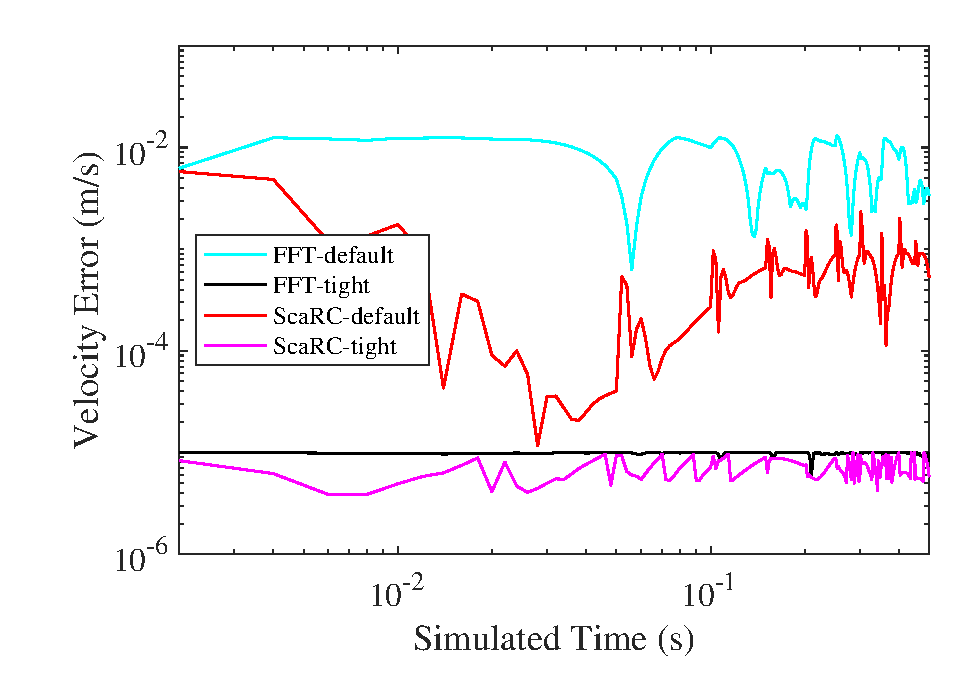
\includegraphics[width=3in]{\figPath/poisson2d_4mesh/poisson2d_4mesh_velerror}\\
\end{center}
\caption[Velocity tolerances of the structured pressure solvers in case of the 4-mesh poisson2d test case]{Velocity tolerances of the structured pressure solvers for a 4-mesh subdivision of the {\ct poisson2d} test case.}
\label{FIG_SCARC_poisson_four_velerror}
\end{figure}

\begin{figure}[h]
\begin{center}
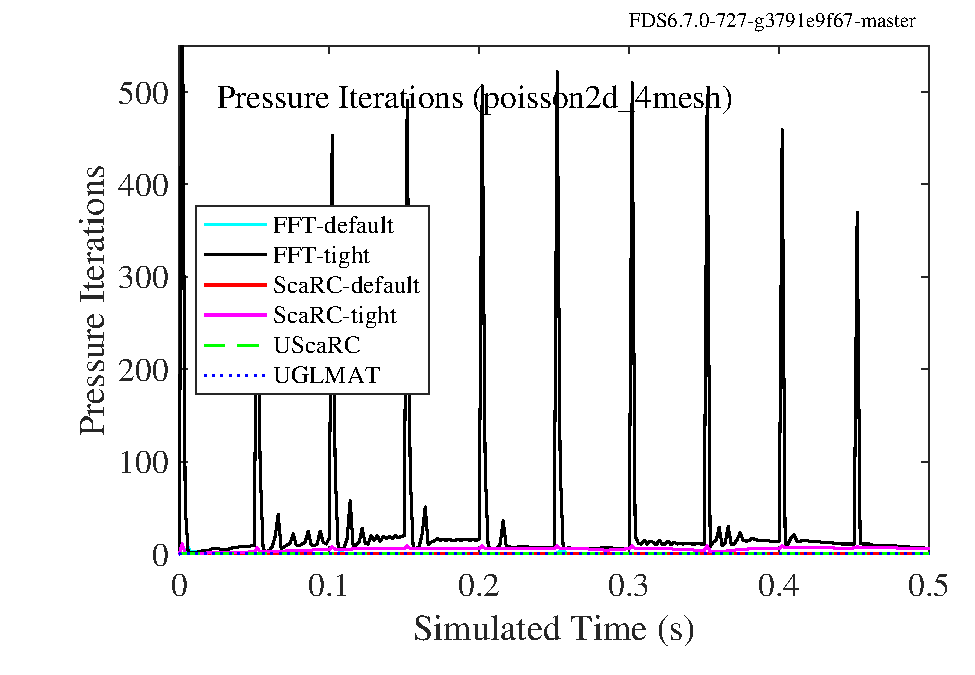
\includegraphics[width=3in]{\figPath/poisson2d_4mesh/poisson2d_4mesh_presite}
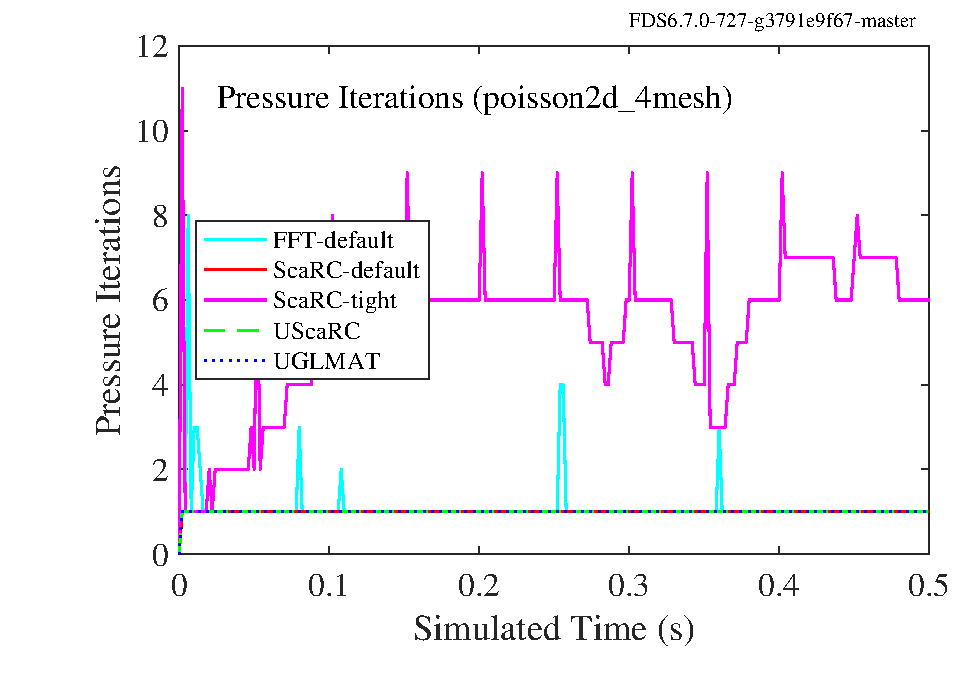
\includegraphics[width=3in]{\figPath/poisson2d_4mesh/poisson2d_4mesh_presite_zoom}
\end{center}
\caption[Pressure iterations of the different pressure solvers for {\ct poisson2d} with 4 meshes]{Pressure iterations of the different pressure solvers for a 4-mesh subdivision of the {\ct poisson2d} test case.  (Left) Comparison of all solvers. (Right) Zoomed view  without \ffttight{}.}
\label{FIG_SCARC_poisson_four_presite}
\end{figure}

According to the size of the default velocity tolerance, \fftdefault{} (cyan) leads to a coarse velocity error in the range of  $10^{-2}$ as can be seen in Figure \ref{FIG_SCARC_poisson_four_velerror}.  
This error consists of two parts, namely the error along the internal obstruction and the error at the mesh interfaces. The related pressure iteration mostly converges within 1 cycle. Only with changing inflow conditions occasionally up to 4 cycles are needed as can be seen at the cyan line in the right plot of Figure \ref{FIG_SCARC_poisson_four_presite}. The maximum number of 8 cycles is only required at the beginning of the simulation until the flow field has built up for the first time, but never again after. Thus, convergence is fast, but it is also associated with the error of the pressure trace displayed in Figure \ref{FIG_SCARC_poisson_four_trace}.

Although its surrounding pressure iteration is based on the same default velocity tolerance, 
\scarcdefault{} (red) already provides a basically smaller velocity error compared to \fftdefault{} in the range of about $10^{-4}$ up to $10^{-3}$, see Figure \ref{FIG_SCARC_poisson_four_velerror} again.
This is because the only part that makes up this error relates to the inner obstruction, whereas nothing is added at mesh interfaces any more.  Convergence can always be achieved in just 1 pressure iteration independently of the inflow changes and there is no major fluctuation at the beginning, see the right plot of Figure \ref{FIG_SCARC_poisson_four_presite}.

Figure \ref{FIG_SCARC_poisson_four_velerror} also proves that
\ffttight{} (black) and \scarctight{} (magenta) in fact succeed to fulfill the required velocity tolerance of $10^{-5}$. 
However, when looking to Figure \ref{FIG_SCARC_poisson_four_presite} the biggest difference between both solvers becomes apparent: While \ffttight{} needs relatively many pressure iterations (averagely 35) to fulfill the fine tolerance, \scarctight{} requires considerably less (averagely 6). 
Note, that the average calculation was restricted to the time interval $[0.05,0.5]$ such that the higher fluctuations which only occur at the beginning were neglected in order not to falsify the whole picture.
In particular, at every change of the inflow conditions, the latency of \ffttight{} gets obvious in a short-term increase of the number of iterations (up to 522 in the worst case) which basically relies on the fragmentation induced by the subdivision. 

The right plot in Figure \ref{FIG_SCARC_poisson_four_presite} also reveals slight increases for \scarctight{} for every inflow change, since it still has to prevent the velocity penetration to the obstruction. However this is significantly less than for \ffttight{} and a maximum of 11 iterations is not exceeded.
This difference again reflects the fact that \scarc{} already captures the subdivision correctly and that the only disturbing influences refer to the internal obstruction. As expected, \uglmat{} (blue dotted) and \uscarc{} (green dashed)
produce machine precision accuracy in exactly one pressure iteration.

\subsection{2D Poisson test case based on a subdivision into 16 meshes}
Subsequently, the {\ct poisson2d} geometry from Figure \ref{FIG_basic_pipe_geometry} is not only subdivided into 4 but into 16 meshes with a side length of 20~cm and $32^2$ cells each (corresponding to the finer grid resolution of 0.625~cm). The resulting flow field is illustrated in Figure \ref{FIG_scarc_poisson_sixteen_flowfield}.

\begin{figure}[ht]
\begin{center}
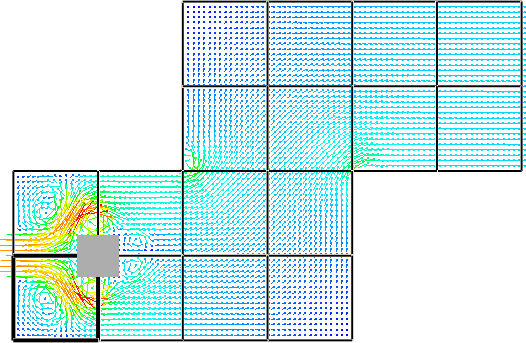
\includegraphics[width=0.6\textwidth]{\figPath/poisson2d_16mesh/poisson2d_16mesh_flowfield}
\end{center}
\caption[Flow field for {\ct poisson2d} with 16 meshes]{Flow field for a 16-mesh subdivision of the {\ct poisson2d} test case at $t=0.31$~s.}
\label{FIG_scarc_poisson_sixteen_flowfield}
\end{figure}

\newpage
As Figure \ref{FIG_scarc_poisson_sixteen_convergence} shows, a fundamental 
improvement of numerical efficiency can be achieved by adding coarse grid information.
The left plot therein displays the slow convergence rates which are achieved for default \scarc{} and \uscarc{} (working both only on fine-grid level), the much better rate for \scarctwolevel{} (working on 2 different grid levels) and the very good rate for \scarcmultigrid{} (working on 3 different grid levels as displayed in Figure \ref{FIG_default_scarc_mg}). The related number of \scarc{} iterations is shown in the right plot of Figure \ref{FIG_scarc_poisson_sixteen_convergence}. 



\begin{figure}[h]
\begin{center}
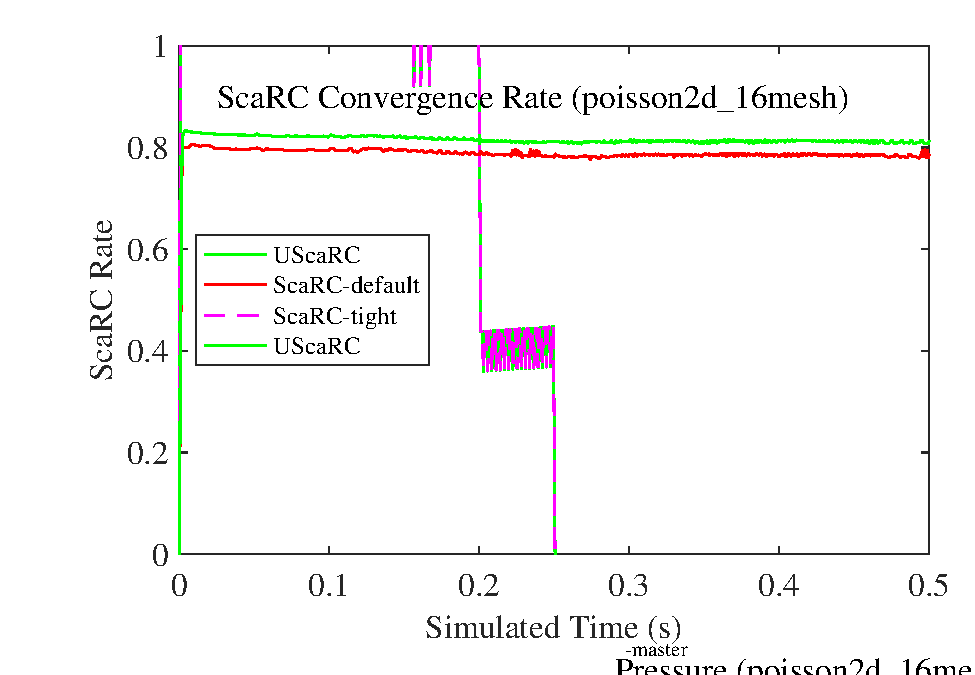
\includegraphics[width=3in]{\figPath/poisson2d_16mesh/poisson2d_16mesh_scarc_rate}
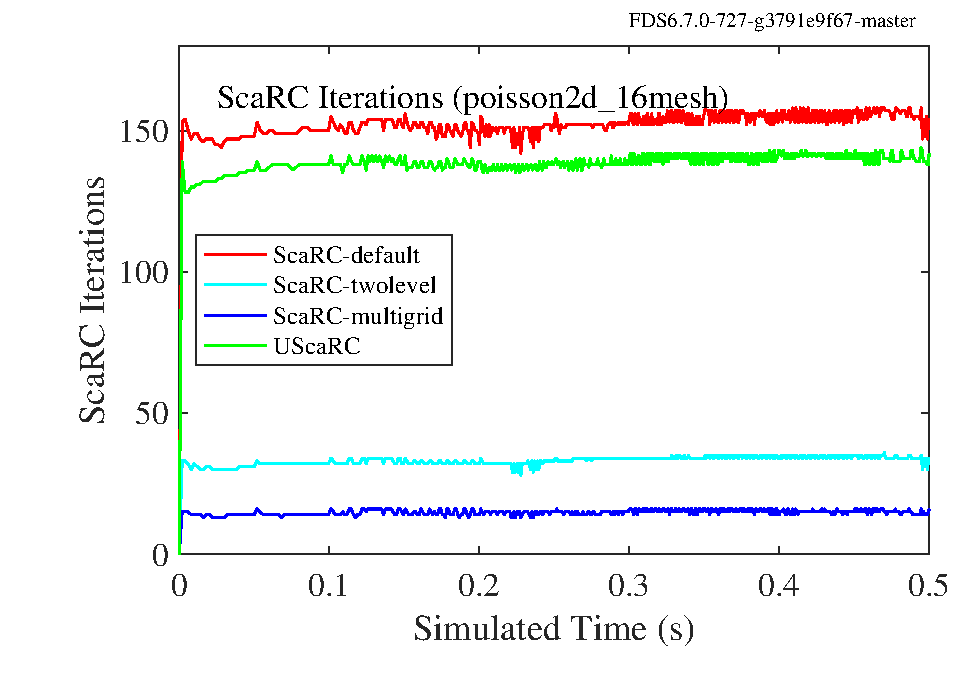
\includegraphics[width=3in]{\figPath/poisson2d_16mesh/poisson2d_16mesh_scarc_iter}
\end{center}
\caption[Comparison of the different \scarc{} variants] {Comparison of different \scarc{} variants for a 16-mesh subdivision of the {\ct poisson2d} test case. (Left) \scarc{} convergence rates.  (Right) Number of required \scarc{} iterations. }
\label{FIG_scarc_poisson_sixteen_convergence}
\end{figure}

When looking to \scarctwolevel{}, the additional usage of a coarser grid level obviously leads to a halving of the convergence rate from 0.81 to about 0.42, see the left plot of Figure \ref{FIG_scarc_poisson_sixteen_convergence}. The right plot therein shows that this reduction is also associated with a comprehensive  reduction of the number of required global \scarc{} iterations from 150 to about 40, which is quite much because it has to be performed twice per FDS time step.  
Even more significant convergence acceleration can be achieved with the \scarcmultigrid{} variant. Here the number of global \scarc{} iterations is reduced by a factor of 10 to about 15 while the final convergence rate is in the range of 0.15.

Please note that if only a 4-mesh subdivision instead of the 16-mesh subdivision is used for the {\ct poisson2d} geometry while maintaining the same fine-grid resolution of 0.625 cm, a convergence rate of 0.7 with about 90 global iterations is achieved for the default \scarc{} and \uscarc{} which still is not very good but significantly better than for the 16-mesh case. This observation reflects the fundamental design property of the 1-level variants that their convergence rate decreases with increasing number of sub-meshes.

This difference is far less pronounced for the two multi-level variants \scarctwolevel{} and \scarcmultigrid{} 
which, due to the use of additional coarse grid information, show convergence rates that are significantly more independent of the number of sub-meshes.

Certainly, the \scarc{} iterations incorporating multiple grid levels are more expensive than the purely 1-level related ones, since additional computations and communications are required. This has to be kept in mind when comparing the different approaches.
All in all, it becomes clear that there is still potential for improvement with regard to the convergence rates of the default \scarc{} variants, but that the use of corresponding coarse grid information points the way and a suitable balance between numerical and parallel efficiency needs to be further worked out here.

\subsection{Summary from the previous test calculations}
\label{SEC_SCARC_poisson_evaluation}

The purpose in developing the {\ct poisson2d} test case was on the one hand to illustrate the functionality of the different \scarc{} variants and on the other hand to prove their basic correctness. The variants shown differ significantly in the type of the underlying discretization, the preconditioning mechanisms used, and whether they work only at the fine grid level or at additional coarser grid levels. 
%
The biggest difference to the current FFT solver consists in the fact that \scarc{} has no more errors along inner mesh boundaries. Thus, for the structured \scarc{} variants often much less pressure iterations are needed than for the default FFT solver, because it only has to reduce the penetration error towards internal obstructions. For the unstructured variant \uscarc{}, no pressure iteration is needed at all.

The previous studies have shown that the addition of coarser grid levels can contribute to a significant improvement of numerical efficiency. However, the achieved convergence acceleration must be put in relation to the increased costs for each single iteration.
A final assessment for the performance of the different variants can only be done on the base of additional measurements of the computational times. 
In order to arrive at meaningful estimates for the optimal parameters a-priori, different sensitivity studies are in work which should finally allow to identify an optimal set of parameters that delivers resilient and efficient results for a large number of general cases.
The coming test series will concentrate on the official FDS verification and validation cases to examine the suitability of \scarc{} for more realistic cases.
